\documentclass{article}
\usepackage{amsmath}
\usepackage{amssymb}
\usepackage{graphicx}
\usepackage{hyperref}
\usepackage[version=4]{mhchem}

\title{Example 1}
\date{}

\begin{document}
\maketitle

(AMC) In triangle \(A B C, B D\) is a median. \(C F\) intersects \(B D\) at \(E\) so that the length of \(B E\) is equal to the length of \(E D\). Point \(F\) is on \(A B\). Then, if \(B F=5, B A\) equals:\\
(A) 10\\
(B) 12\\
(C) 15\\
(D) 20\\
(E) none of these

Solution: (C).\\
\centering
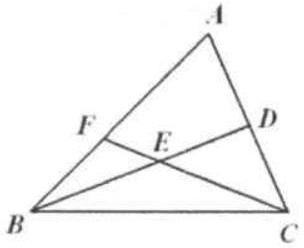
\includegraphics[width=\textwidth]{images/problem_image_1.jpg}

Take \(G\), the midpoint of \(F C\). Connect \(D G . D G / / A F\) and \(D G\) is the midline of triangle \(C A F, D G=\frac{1}{2} A F\).\\
\(\triangle B E F \cong \triangle D E G,(B E=E D, \angle E B F=\angle E D G, \angle B E F\)\\
\(=\angle D E G)\). So \(D G=B F=5, A F=2 D G=10\).\\
Thus \(B A=B F+A F=5+10=15\).\\
\centering
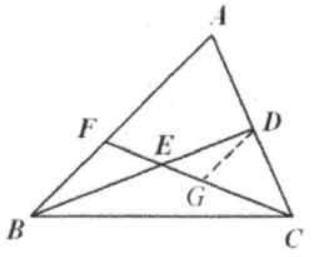
\includegraphics[width=\textwidth]{images/reasoning_image_1.jpg}

The answer is (C).\\

\end{document}
